\documentclass[aspectratio=169]{beamer}
\usetheme{Madrid}
\usepackage[utf8]{inputenc}
\usepackage[T1]{fontenc}
\usepackage{tikz}
\usepackage{amssymb}
\usepackage{graphicx}
\setbeamertemplate{navigation symbols}{}
\setbeamercolor{title}{fg=white,bg=blue!70!cyan}
\setbeamercolor{frametitle}{fg=white,bg=blue!70!cyan}
\setbeamercolor{block title}{bg=blue!70!cyan!20,fg=black}
\setbeamercolor{block body}{bg=blue!70!cyan!8,fg=black}
\setbeamercolor{item}{fg=blue!70!cyan}
\setbeamercolor{itemize item}{fg=blue!70!cyan}
\setbeamertemplate{itemize item}[triangle]

\title{Tier 1 — Sequencing}
\subtitle{Your code does EXACTLY what you write, in EXACTLY that order}
\author{ByteForge --- Grade 9 --- The Deep Diver}
\date{}

\begin{document}

\begin{frame}
    \titlepage
\end{frame}

\begin{frame}{Today's Missions}
    \Large
    \begin{itemize}
        \item Dock at the Station
        \item Around the Wall
        \item Steering Damaged
    \end{itemize}
\end{frame}

\begin{frame}{Sequence: a program is a list, done in order}
    \large
    \begin{itemize}
        \item \texttt{forward(d)} moves in the direction you currently face
        \item \texttt{left(90)}/\texttt{right(90)} rotate on the spot, no movement
        \item Real code now, not blocks --- exact punctuation has to be right
    \end{itemize}
\end{frame}


\begin{frame}{Planning around an obstacle}
    \large
    \begin{itemize}
        \item Read the WHOLE scene before writing a single line
        \item The shortest-LOOKING route can be completely wrong if a wall is in the way
        \item Touching a wall is a genuine mission failure, like a real crash
    \end{itemize}
\end{frame}


\begin{frame}{Working within a real constraint}
    \large
    \begin{itemize}
        \item Steering "damaged" --- only forward()/backward() available, no turning
        \item The right tool is not always the familiar one --- back up, do not try to turn around
    \end{itemize}
\end{frame}

\begin{frame}{Real-World Examples}
    \large
    \begin{itemize}
        \item A GPS giving turn-by-turn directions is a real sequence: exact steps, exact order, no skipping ahead.
    \end{itemize}
\end{frame}


\begin{frame}{Image}
    \begin{center}
    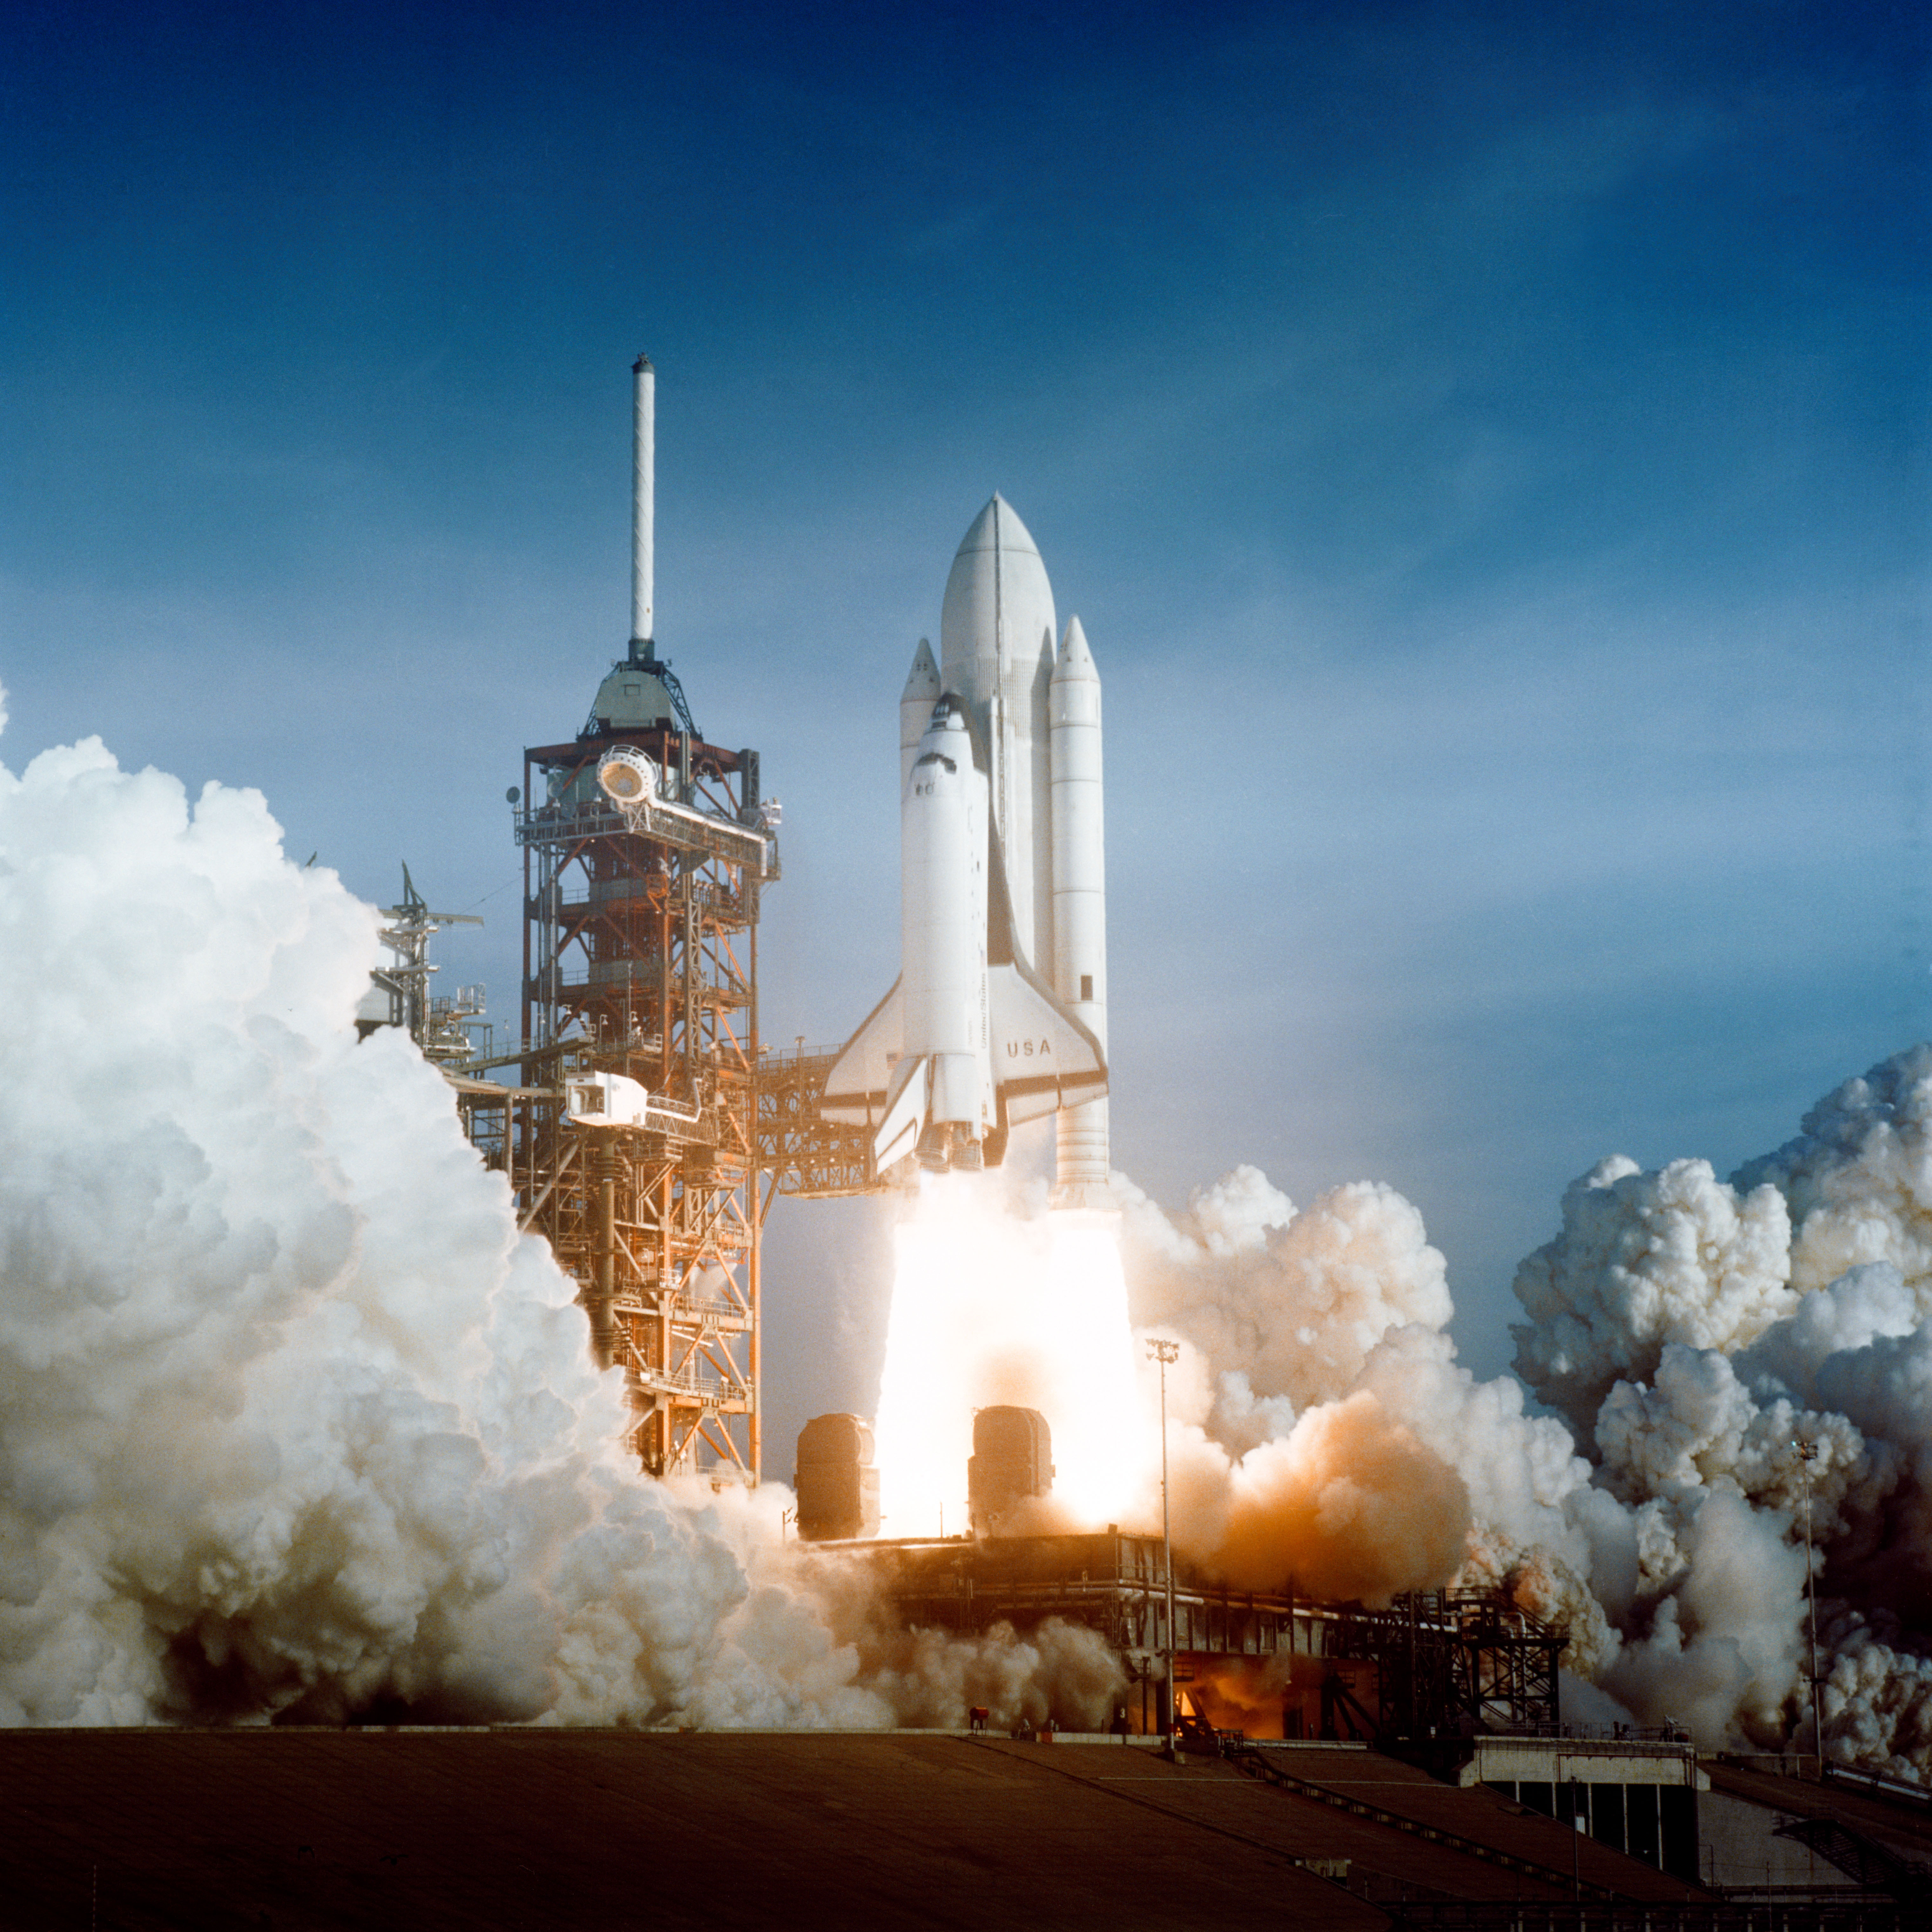
\includegraphics[width=0.5\textwidth]{images/rocket.jpg}

    \large Every mission in this tier is you writing the real flight sequence for a real vehicle --- exactly the same discipline a real launch needs.

    \small Space Shuttle launch --- NASA, public domain, via Wikimedia Commons
    \end{center}
\end{frame}

\begin{frame}{Let Them Discover}
    \large
    On paper, write the exact sequence of forward/turn instructions to get from your classroom door to your own desk. Could someone who has never been in the room follow it perfectly?
\end{frame}

\begin{frame}{Your Turn}
    \Large
    Open the mission map, find \textbf{Tier 1 — Sequencing}, and fly it for real ---
    everything you just saw, you now do yourself.
\end{frame}

\end{document}
